% =====================================================================
%  Estrutura Produtiva do Espírito Santo: uma análise de insumo-produto
%  Felipe Carvalho — PPGEco/UFES — Análise de Insumo-Produto (2026/1)
%
%  Números reproduzíveis de pesquisa/17_caracterizacao_es_2008.py (C1),
%  18_trajetoria_n68.py (C2) e 20_caracterizacao_micro.py (C3).
% =====================================================================
\documentclass[11pt,a4paper]{article}
\usepackage[utf8]{inputenc}
\usepackage[T1]{fontenc}
\renewcommand{\abstractname}{Resumo}
\renewcommand{\refname}{Referências}
\usepackage{amsmath,amssymb}
\usepackage{booktabs}
\usepackage{graphicx}
\usepackage{geometry}
\usepackage{xcolor}
\usepackage[round,authoryear]{natbib}
\usepackage[hidelinks]{hyperref}
\geometry{margin=2.5cm}
\graphicspath{{../pesquisa/outputs/}{../figuras/}}

\title{\textbf{Estrutura Produtiva do Espírito Santo:\\ uma análise de insumo-produto}\\[2pt]
\large Multiplicadores, setores-chave, vocação territorial e abertura de uma
economia de base (2008--2021)}
\author{Felipe Carvalho\\
\small PPGEco --- UFES \quad$\cdot$\quad Análise de Insumo-Produto --- Prof. Dr. Celso Bissoli Sessa}
\date{julho de 2026}

\begin{document}
\maketitle
\thispagestyle{empty}

\begin{abstract}
\noindent
Este artigo caracteriza a estrutura produtiva do Espírito Santo (ES) pela ótica
insumo-produto, na tradição brasileira de análise de economias estaduais. A partir
da matriz insumo-produto inter-regional ES\,$\times$\,restante do Brasil de 2008
(26 setores, com vetor de emprego), da série nacional de 68 setores (2010--2021) e
do sistema inter-regional das dez microrregiões de planejamento (2015), aplica-se a
bateria padrão do método: multiplicadores de produção, emprego e renda (tipos I e
II), ligações de Rasmussen-Hirschman, ligações puras (Guilhoto-Sonis-Hewings),
coeficiente de variação e quocientes locacionais. O retrato é de uma
\emph{economia de base}: os setores líderes --- mineração, petróleo e gás,
siderurgia e celulose --- são grandes, a montante, exportadores e intensivos em
capital, e concentram os maiores multiplicadores de produção (média 1,76 no tipo I)
e as maiores ligações puras (mineração e metalurgia respondem pelos maiores polos),
mas \textbf{geram pouco emprego e renda diretos}: a geração de empregos concentra-se
em setores trabalho-intensivos (têxtil, pecuária, serviços) e a de renda, em
serviços e administração pública. A estrutura é \emph{dual}: a extração (petróleo e
minério de ferro) opera como \emph{enclave} de baixa ligação doméstica (ligação para
trás inferior à unidade), enquanto a transformação (siderurgia, celulose, refino) é
setor-chave; ao longo de 2010--2021, a celulose adensa, a siderurgia oscila e a
extração permanece enclave. Um benchmark com as 27 unidades da federação mostra que essa
dualidade é \emph{genérica} ao método, mas que o ES é um de seus \emph{casos-limite} --- o
segundo estado mais intensivo em setores de base e um dos de menor multiplicador de emprego.
Essa base é, ademais, \emph{hiperaberta}: 24,9\% do multiplicador vaza para fora do estado, o
\emph{spillover} escoa concentrado ao núcleo São Paulo--Rio (52,5\%) com \emph{feedback} de
apenas 0,32\%, e essa lógica-plataforma reproduz-se, em \emph{escalas aninhadas}, entre as microrregiões.
No território, o estado é um \emph{mosaico de vocações}:
um núcleo metropolitano diversificado cercado por microrregiões especializadas
(celulose no Rio Doce, rochas ornamentais no Central Sul, pelotização no Litoral Sul,
têxtil no Centro-Oeste, agropecuária nas serranas).

\vspace{0.6em}
\noindent\textbf{Palavras-chave:} insumo-produto; estrutura produtiva; multiplicadores;
setores-chave; economia regional; Espírito Santo.

\noindent\textbf{Códigos JEL:} R15; D57; C67.
\end{abstract}

% =====================================================================
\section{Introdução}
\label{sec:intro}
O Espírito Santo respondia, em 2008, por cerca de 2\% do produto nacional, mas sua
estrutura produtiva é atípica: pequena, hiperaberta e organizada em torno de
\emph{commodities} industriais de grande escala e intensivas em recursos naturais ---
minério de ferro e pelotização, siderurgia, petróleo e gás, celulose e rochas
ornamentais. Em menos de quatro décadas, a economia capixaba trocou de motor duas
vezes: da monocultura cafeeira para a indústria de base nos anos 1980 (os grandes
projetos siderúrgico, de celulose e de pelotização) e, a partir do fim dos anos 1990,
para o petróleo, hoje cerca de um quarto do produto estadual.

A escola brasileira de insumo-produto consolidou um formato para \emph{caracterizar}
uma economia estadual: a partir de uma matriz inter-regional (estado \emph{versus}
restante do país), computam-se multiplicadores, ligações intersetoriais e
setores-chave, identificando o perfil de especialização e os centros de dinamismo.
Esse formato foi aplicado a diversos estados --- Mato Grosso
\citep{figueiredo2004agriculture}, Rio Grande do Sul \citep{porsse2008matriz},
entre outros. Para o Espírito Santo, há contribuições \emph{pontuais}:
\citet{sessa2017ubu} avaliam o impacto socioeconômico de um projeto siderúrgico (a
Companhia Siderúrgica de Ubu, em Anchieta) pela matriz capixaba, e \citet{ribeiro2024dinamica}
regionalizam a matriz de 2015 nas dez microrregiões de planejamento, computando
multiplicadores de produção, emprego e renda. Falta, contudo, uma \textbf{caracterização
estrutural abrangente} --- que reúna a bateria completa de indicadores, um \emph{benchmark}
interestadual que separe o específico do genérico e um pano de fundo temporal ---,
lacuna que este artigo preenche,
respondendo a três perguntas descritivas: (i) \emph{que tipo de economia} é o ES ---
quais seus multiplicadores, setores-chave e polos de crescimento (\S\ref{sec:retrato});
(ii) \emph{como} a posição estrutural de seus setores de base evoluiu no tempo
(\S\ref{sec:panorama}); e (iii) \emph{qual a vocação} de cada um de seus territórios
(\S\ref{sec:territorio}). A contribuição não é testar uma hipótese, mas oferecer um
retrato insumo-produto sistemático --- e reprodutível --- da economia capixaba.

% =====================================================================
\section{Dados}
\label{sec:dados}
A análise combina três fontes, todas processadas por rotinas reprodutíveis
(\texttt{pesquisa/}): (a) a matriz \textbf{inter-regional ES\,$\times$\,restante do
Brasil} de 2008, 26 setores por região, R\$ milhões correntes, balanceada e
acompanhada dos vetores de remunerações e de pessoal ocupado, que sustenta o retrato
estrutural; (b) a \textbf{série nacional de 68 setores} (2010--2021), do sistema de
matrizes do NEREUS/USP, que permite a leitura temporal; e (c) o \textbf{sistema
inter-regional das dez microrregiões de planejamento do ES} (2015, 35 setores), que
sustenta a caracterização territorial. A construção das matrizes regionais segue a
tradição brasileira de regionalização não-censitária da matriz nacional
\citep{guilhoto2005estimacao,round1983nonsurvey} pelo método IIOAS
\citep{haddad2017iioas}. As heterogeneidades de safra (2008/2015) e agregação
(26/35/68 setores) e o caráter \emph{estimado} dos fluxos inter-regionais são
discutidos em \S\ref{sec:limites}.

% =====================================================================
\section{Método}
\label{sec:metodo}
O sistema parte da identidade de Leontief $x=(I-A)^{-1}y=By$, com $A=Z\hat{x}^{-1}$.
Sobre $B$ (e, pelo lado da oferta, sobre a inversa de Ghosh $G$) computa-se a bateria
de indicadores que caracteriza uma economia regional \citep{millerblair2009}.

\paragraph{Multiplicadores.}
O multiplicador de produção do setor $j$ é $O_j=\sum_i b_{ij}$. Os de emprego e renda
são $E_j=\sum_i w_i b_{ij}$ e $R_j=\sum_i v_i b_{ij}$, com coeficientes diretos
$w_i=\text{ocup}_i/x_i$ e $v_i=\text{rem}_i/x_i$. Os multiplicadores de \emph{tipo II}
fecham o modelo para as famílias \emph{do ES} (renda das remunerações dos setores capixabas;
consumo das famílias capixabas), endogeneizando o efeito-renda induzido. Num sistema bi-regional,
essa escolha fornece um \emph{limite inferior} do induzido capixaba, pois parte do consumo das
famílias se realiza em produtos do restante do Brasil e não retorna como demanda ao ES.

\paragraph{Ligações e setores-chave.}
Os índices de \citet{rasmussen1956} e \citet{hirschman1958} medem o poder de dispersão
(para trás, pela inversa de Leontief) e a sensibilidade de dispersão (para frente, pela
inversa de Ghosh), normalizados pela média; \emph{setores-chave} têm ambos os índices
superiores à unidade. O coeficiente de variação desses índices mede o grau de
integração da economia.

\paragraph{Ligações puras.}
Como a normalização de Rasmussen-Hirschman é neutra ao tamanho do setor, computam-se
também as \emph{ligações puras} (Guilhoto-Sonis-Hewings; \citealp{millerblair2009}),
que ponderam o encadeamento pela produção do setor. Particionando a economia em
$\{j\}$ e o resto $\{r\}$, a ligação pura para trás é
$\mathrm{PBL}_j=\Delta^{r}A^{rj}\Delta^{j}y_j$ e a ligação pura para frente,
$\mathrm{PFL}_j=\Delta^{j}A^{jr}\Delta^{r}y_r$, com $\Delta^{r}=(I-A^{rr})^{-1}$ e
$\Delta^{j}=(1-a_{jj})^{-1}$; a ligação pura total $\mathrm{PTL}_j$ identifica os reais
polos de crescimento.

\paragraph{Vocação territorial.}
A especialização de cada microrregião é medida pelo \emph{quociente locacional}
$\mathrm{LQ}_{gs}=(x_{gs}/\sum_s x_{gs})/(\sum_g x_{gs}/\sum_{gs}x_{gs})$; valores
acima da unidade indicam concentração do setor $s$ no território $g$ acima da média
estadual.

\paragraph{Abertura: \emph{spillover} e \emph{feedback}.}
Para medir a abertura, particiona-se o sistema em região-foco $L$ e resto $M$ e aplica-se
a decomposição de Isard \citep{isard1951,millerblair2009}. Injetando a demanda final de $L$
por seus próprios produtos, a produção induzida em $M$,
$x^{M}=(I-A^{MM})^{-1}A^{ML}x^{L}$, é o \emph{spillover}; o retorno a $L$ pelo termo de
\emph{feedback} da inversa particionada $(I-A^{LL}-A^{LM}(I-A^{MM})^{-1}A^{ML})^{-1}$ é o
\emph{feedback}. A razão \emph{feedback}/injeção, computada em cada escala (UFs e
microrregiões), mede a reciprocidade do encadeamento.

% =====================================================================
\section{O retrato estrutural (2008)}
\label{sec:retrato}
\paragraph{Multiplicadores.}
O multiplicador de produção médio dos 26 setores do ES é 1,76 (tipo I) e 2,45 (tipo
II). Os mais altos estão na indústria de transformação --- alimentos (2,31), refino
(2,11), material de transporte (2,10) e químicos (2,10). O contraste com os
multiplicadores de \emph{emprego} é o achado central do retrato: a geração de empregos
(27,9 por R\$ 1 milhão de demanda final, no tipo I) concentra-se em setores
\emph{trabalho-intensivos} --- têxtil (67,9), pecuária (57,0), alojamento (50,2),
serviços (49,2) e agricultura (46,7) ---, \emph{nenhum} deles um setor de base. A
geração de renda das famílias, por sua vez, é maior em educação, administração
pública, saúde e serviços. Os setores que lideram a economia capixaba não são os que
mais empregam nem os que mais distribuem renda diretamente.

\paragraph{Setores-chave e polos de crescimento.}
Pela classificação de Rasmussen-Hirschman, os setores-chave (ambos os índices acima de
1) são a cadeia industrial de transformação: refino, químicos, borracha/plástico,
cimento e minerais não-metálicos, metalurgia, material elétrico, material de transporte
e eletricidade/gás/água (Figura~\ref{fig:chave}). A mineração, notavelmente, tem
\emph{ligação para frente} elevada ($\approx1{,}2$) mas \emph{ligação para trás}
baixa ($\approx0{,}9$): é fornecedora a montante, não setor-chave pleno --- a
assinatura de um \emph{enclave} que compra pouco internamente. Já as ligações puras,
ponderadas por tamanho, identificam os verdadeiros polos: \textbf{mineração}
($\mathrm{PTL}$ padronizado 4,4) e \textbf{metalurgia} (3,4) à frente, seguidas de
transporte, comércio e serviços.\footnote{A ligação pura total correlaciona-se fortemente
com o valor bruto da produção (Pearson 0,96): é, sobretudo, uma medida de \emph{tamanho}.
Seu acréscimo sobre o VBP cru está na \emph{reordenação pela conexão} --- promove acima do
que o porte diria setores bem articulados mas não os maiores (madeira/papel, cimento,
eletricidade) ---, e por isso é reportada ao lado de Rasmussen-Hirschman, neutra ao porte.}
O grau de integração (coeficiente de variação das
ligações) é moderado: 0,16 para trás, 0,28 para frente.

\begin{figure}[ht]
\centering

\includegraphics[width=.92\linewidth]{fig_setores_chave.png}
\caption{Mapa de ligações dos 26 setores do ES (2008). O quadrante superior-direito
(vermelho) reúne os setores-chave (poder e sensibilidade de dispersão acima da média);
a mineração aparece como forte fornecedora a montante, com baixa ligação para trás.}
\label{fig:chave}
\end{figure}

\paragraph{O ES é típico ou extremo? Um benchmark interestadual.}
Que a extração tenha baixa ligação para trás é uma regularidade \emph{universal} do método ---
mineração e petróleo são pobres em insumos intermediários em qualquer economia. A pergunta
relevante não é \emph{se} o ES exibe a dualidade, mas se a exibe de forma \emph{distintiva}.
Comparando o ES às 27 unidades da federação na matriz interestadual de 2008
(Tabela~\ref{tab:bench}), a resposta é precisa: a dualidade é \textbf{genérica em tipo, mas
extrema em grau}.\footnote{Os valores da Tabela~\ref{tab:bench} são médias \emph{ponderadas pela
produção} sobre a matriz \emph{interestadual} (27 UFs), escolha que garante comparabilidade entre
estados; diferem, por isso, das médias \emph{simples} sobre a matriz \emph{bi-regional} reportadas
no início desta seção (produção 1,76; emprego 27,9). As duas descrevem o mesmo fenômeno sob
agregações distintas.} Nos indicadores neutros à composição --- multiplicador de produção (1,66; 14\textordmasculine)
e ligação para trás ponderada (0,92; 14\textordmasculine) --- o ES é \emph{exatamente mediano}. É na
\emph{composição} e no \emph{emprego} que ele se destaca: é o \textbf{segundo} estado mais intensivo em
setores de base (36,4\%, só atrás de Mato Grosso) e está entre os de \textbf{menor} multiplicador de
emprego (25,4 empregos por R\$ milhão; 24\textordmasculine\ de 27). O sintoma mais nítido: o emprego
gerado por seu setor dominante equivale a apenas 39\% da média estadual --- o \textbf{segundo} valor
mais baixo do país (mediana 65\%). O Espírito Santo não é, pois, um contraexemplo da regularidade, mas
um de seus \emph{casos-limite}: a economia onde a base extrativa-industrial pesa mais e menos emprego
direto distribui.

\begin{table}[ht]
\centering\small
\begin{tabular}{lrrr}
\toprule
Métrica & ES & posição & mediana (27 UFs) \\
\midrule
Participação de setores de base (\%) & 36,4 & 2\textordmasculine & 21,0 \\
Multiplicador de produção (pond.) & 1,66 & 14\textordmasculine & 1,66 \\
Multiplicador de emprego (empr./R\$\,mi) & 25,4 & 24\textordmasculine & 42,5 \\
Ligação para trás (pond.) & 0,92 & 14\textordmasculine & 0,92 \\
Emprego do líder $\div$ média estadual & 0,39 & 2\textordmasculine\ mais baixo & 0,65 \\
\bottomrule
\end{tabular}
\caption{O ES entre as 27 UFs (2008): mediano nos indicadores neutros à composição, extremo na
intensidade de base e na pobreza de emprego dos líderes. Fonte:
\texttt{22\_benchmark\_caracterizacao.py}.}
\label{tab:bench}
\end{table}

% =====================================================================
\section{O panorama temporal (2010--2021)}
\label{sec:panorama}
Uma ressalva de objeto antecede esta seção. O Espírito Santo dispõe apenas de \emph{âncoras}
insumo-produto --- 2008 (estadual) e 2015 (microrregional) ---, não de uma série anual própria.
O que a série nacional de 68 setores (2010--2021) oferece não é, portanto, a trajetória da
\emph{estrutura capixaba}, e sim o \textbf{pano de fundo nacional} dos setores que a definem:
como evoluiu, no país, a posição estrutural da extração, da siderurgia, do refino e da celulose ---
os ramos sobre os quais a economia do ES está montada. É uma leitura de tendência \emph{dos setores},
não \emph{do estado}; lida assim, ela é informativa e honesta (Figura~\ref{fig:traj}). A leitura
confirma, ao longo do tempo, a \emph{dualidade} do retrato de 2008. A \textbf{celulose e papel} é o
setor-chave mais consistente e em fortalecimento --- sua ligação para trás sobe de 1,41
(2010) a 1,51 (2021) e seu multiplicador de produção, de 2,85 a 3,05. A
\textbf{siderurgia} é setor-chave na maior parte do período (ligação para trás entre
1,2 e 1,4), com um recuo em 2021 que merece cautela interpretativa: a queda concentra-se
na cadeia metálica (ferro-gusa, metais não-ferrosos, produtos de metal) e é coerente com
o \emph{salto de preços do aço} em 2021 incidindo sobre matrizes a preços correntes ---
quando o valor da produção sobe mais que as compras intermediárias, o coeficiente técnico
$a_{ij}=z_{ij}/x_j$ cai por efeito nominal, não por desintegração estrutural. O
\textbf{refino} mantém-se no limiar de setor-chave. Já a \textbf{extração de petróleo e gás} e a \textbf{extração de minério
de ferro} operam como enclaves: sua ligação para trás permanece \emph{abaixo da
unidade} em quase todos os anos --- compram poucos insumos domésticos ---, e o minério
de ferro registra seu pico de integração justamente em 2015--2016, em torno do
rompimento de Fundão, recuando em seguida. A transformação carrega os encadeamentos; a
extração os dispensa.

\begin{figure}[ht]
\centering

\includegraphics[width=.95\linewidth]{fig_trajetoria_n68.png}
\caption{Ligação para trás dos setores-base do ES na estrutura nacional, 2010--2021
(série de 68 setores). Celulose e siderurgia acima da unidade (setores-chave); extração
de petróleo e de minério abaixo (enclaves de baixa ligação doméstica).}
\label{fig:traj}
\end{figure}

% =====================================================================
\section{A vocação territorial (2015)}
\label{sec:territorio}
O sistema das dez microrregiões revela um \emph{mosaico de vocações}
(Figura~\ref{fig:vocacao}). A Região Metropolitana (Grande Vitória) concentra 62\% da
produção estadual e é o núcleo diversificado --- petróleo, siderurgia (a usina de
Tubarão) e serviços. Ao seu redor, territórios especializados, cada qual com um
quociente locacional elevado em seu setor: \textbf{celulose} no Rio Doce
($\mathrm{LQ}\,8{,}2$; corredor Linhares/Aracruz), \textbf{rochas ornamentais} no
Central Sul ($\mathrm{LQ}\,7{,}7$; Cachoeiro de Itapemirim), \textbf{minério de ferro e
pelotização} no Litoral Sul ($\mathrm{LQ}\,9{,}5$; Anchieta), \textbf{têxtil} no
Centro-Oeste ($\mathrm{LQ}\,9{,}6$; Colatina) e um interior \textbf{agropecuário} nas
serranas e no Caparaó --- com destaque para a pecuária/avicultura na Central Serrana
($\mathrm{LQ}\,21{,}9$; Santa Maria de Jetibá). A economia capixaba não é homogênea: é
um núcleo industrial-exportador cercado por especializações regionais nítidas.
Um padrão menos óbvio que o mapa de especialização emerge ao medir a \emph{concentração}
da composição setorial de cada microrregião (índice de Herfindahl): ela não acompanha o
porte (correlação $\approx0$), mas a \emph{vocação} --- os territórios extrativos (Litoral
Sul, minério, HHI 0,18; Nordeste, petróleo, 0,14) são os mais mono-estruturais, reproduzindo
na escala territorial o mesmo padrão-\emph{enclave} que a extração exibe na escala setorial,
ao passo que o núcleo metropolitano é diversificado.
Esta leitura dialoga com \citet{ribeiro2024dinamica}, que regionalizaram a mesma matriz de
2015 e identificaram setores-chave por microrregião (alimentos, eletricidade, minerais
não-metálicos) pela geração de emprego e renda; o quociente locacional aqui adiciona a esse
retrato a dimensão da \emph{especialização} --- não apenas onde os multiplicadores são altos,
mas em que cada território é, comparativamente, especializado ---, e os dois resultados
convergem para o mesmo desenho de um estado polarizado entre núcleo e periferias vocacionadas.

\begin{figure}[ht]
\centering

\includegraphics[width=\linewidth]{fig_micro_vocacao.png}
\caption{Quociente locacional por setor e microrregião (2015). Cada território
concentra (vermelho) o setor de sua vocação; a Metropolitana, diversificada, não exibe
especialização extrema.}
\label{fig:vocacao}
\end{figure}

% =====================================================================
\section{Abertura, vazamento e a face plataforma}
\label{sec:plataforma}
Caracterizada a estrutura --- setorial, temporal e territorial ---, resta a dimensão que a
\emph{conecta} ao resto do país: a abertura. Aqui a economia de base revela-se também uma
\emph{economia-plataforma}, no sentido de que seu encadeamento se realiza, em boa parte, fora
do estado.

\paragraph{Vazamento.} Em média, \textbf{24,9\%} do multiplicador de produção capixaba vaza
para fora do ES (22,9\% na média ponderada pela produção). No emprego, o vazamento dos setores
pesados é ainda maior --- metade ou mais do trabalho que a demanda capixaba mobiliza realiza-se
fora do estado: refino 61,6\%, alimentos 56,5\%, madeira/papel 50,3\% e metalurgia 49,3\%.

\paragraph{\emph{Spillover} e \emph{feedback}.} Uma injeção de R\$\,51,5 bilhões na demanda
final do ES por produtos do ES transborda R\$\,18,2 bilhões de produção para o restante do país
(35\% da injeção), mas o \emph{feedback} de volta é de apenas R\$\,164 milhões ---
\textbf{0,32\%}. A interdependência é quase unilateral. E o destino é concentrado: o
\textbf{Sudeste} (excluído o ES) absorve \textbf{65\%} do \emph{spillover}, e o núcleo São
Paulo--Rio de Janeiro, \textbf{52,5\%}. O ES alimenta seus vizinhos mais ricos; o encadeamento
que escapa é capturado a jusante e quase não retorna.

\paragraph{Invariância de escala.} Essa lógica-plataforma não é idiossincrática do ES perante o
Brasil --- ela \emph{se reproduz dentro} do estado. A razão de \emph{feedback} cresce com o
porte da unidade nas duas escalas: $R^2=0{,}59$ entre as 27 UFs e $R^2=0{,}91$ entre as 10
microrregiões (Figura~\ref{fig:fractal2}). A Região Metropolitana retém o multiplicador
(vazamento de 8,4\%, 62\% da produção estadual), enquanto a periferia primário-exportadora vaza
encadeamento \emph{para a metrópole} (até 76\% de seu \emph{spillover}). O par retém-no-núcleo /
vaza-da-periferia configura, pois, uma relação \emph{núcleo-periferia aninhada}
\citep{friedmann1966}: a periferia está para o ES como o ES está para o
Sudeste --- a mesma assinatura de \emph{enclave} que a concentração territorial já indicava
(\S\ref{sec:territorio}), agora pelo lado do fluxo. A pequenez do \emph{feedback} é, em parte,
regularidade de porte \citep{miller1966}; o que é próprio do ES, como mostra o benchmark, é a
\emph{intensidade} com que a exibe.

\begin{figure}[ht]
\centering
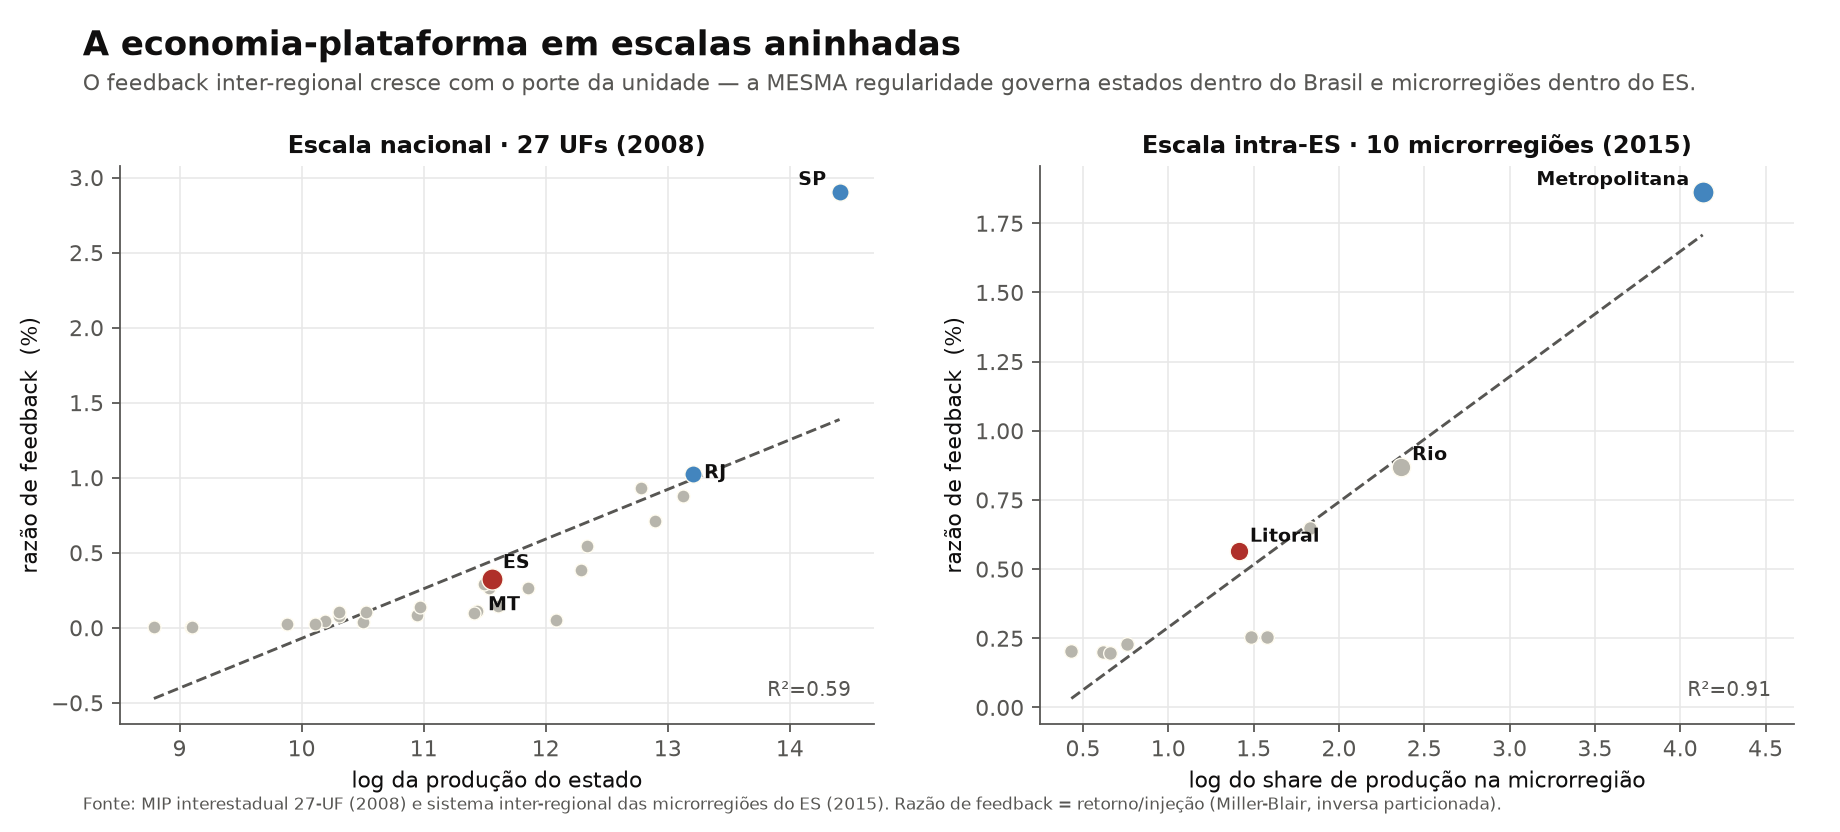
\includegraphics[width=\linewidth]{fractal_duas_escalas.png}
\caption{Invariância de escala da razão de \emph{feedback}: cresce com o porte da unidade nas
duas escalas --- 27 UFs no Brasil ($R^2=0{,}59$) e 10 microrregiões no ES ($R^2=0{,}91$). A
mesma mecânica de posição-e-porte opera em ambas. Fonte: \texttt{14\_*} e \texttt{15\_*}.}
\label{fig:fractal2}
\end{figure}

% =====================================================================
\section{Discussão}
\label{sec:discussao}
O conjunto desenha o ES como uma \textbf{economia de base, dual e pouco geradora de
trabalho direto em seus setores líderes}. Esse perfil dialoga com o debate
brasileiro sobre \emph{desindustrialização} e \emph{primarização} da estrutura produtiva ---
debate que a literatura nacional de insumo-produto examinou com as \emph{mesmas} ferramentas
aqui empregadas. \citet{morceiro2012} documenta, por multiplicadores de Rasmussen-Hirschman e
indicadores de conteúdo importado, a erosão dos encadeamentos da indústria brasileira; já
\citet{nassif2015}, pelos índices de ligação entre 1996 e 2009, relativizam a tese e encontram
pouca evidência de desindustrialização agregada --- no plano nacional, o debate permanece em
aberto. A contribuição do caso capixaba não é arbitrá-lo, mas mostrar, na escala estadual, uma
economia já estruturalmente \emph{especializada em base}: o ES exibe de forma concentrada o
perfil de baixa ligação doméstica e baixa geração de emprego que a literatura de
desindustrialização \citep{oreiro2010} e de doença holandesa \citep{cordenneary1982} associa às
economias intensivas em recursos --- e o benchmark confirma que o faz de modo particularmente agudo. Os setores que a definem --- mineração,
petróleo, siderurgia, celulose --- têm grande porte, alta ligação para frente e os
maiores polos de crescimento pela medida de ligações puras; mas é a sua condição de
fornecedores a montante, e não de articuladores a jusante, que se destaca. A
consequência distributiva é direta: o emprego e a renda diretos vêm de outros setores
(trabalho-intensivos e serviços), de modo que o dinamismo da base não se traduz
automaticamente em ocupação. A essa fragilidade setorial soma-se uma fragilidade
\emph{geográfica}: como mostra a face plataforma (\S\ref{sec:plataforma}), o encadeamento que
a base gera \emph{vaza} para o núcleo SP--RJ com retorno quase nulo --- a captura de valor não
é só um problema de \emph{composição} setorial, mas também de \emph{posição} na hierarquia
regional, e essa lógica repete-se, em escala aninhada, da periferia capixaba para a Grande Vitória.
A dualidade entre extração-enclave e
transformação-chave, visível no retrato de 2008 e persistente na série 2010--2021,
sugere que o adensamento de cadeia tem mais a ganhar na transformação (siderurgia,
celulose) do que na extração, cujos elos domésticos são estruturalmente rarefeitos. No
território, o mosaico de vocações indica que uma política de diversificação produtiva
precisa de endereço sub-estadual: o desafio do núcleo metropolitano (adensar a
indústria de base) é distinto do desafio das microrregiões especializadas (agregar
valor à celulose, às rochas, ao agro). Três alavancas emergem do próprio dado. \textbf{(i) Adensar a jusante da base mineral}: a
mineração e a siderurgia têm as maiores ligações puras (4,4 e 3,4) mas a metalurgia já é
setor-chave e a fabricação de produtos de metal tem multiplicador elevado --- estender a cadeia
minério\,$\to$\,aço\,$\to$\,produtos de metal retém, internamente, encadeamento que hoje escoa.
\textbf{(ii) Apostar na celulose}, o único setor-base cuja ligação para trás \emph{cresce} na
série nacional (1,41\,$\to$\,1,51): é o ramo de base com a trajetória estrutural mais favorável.
\textbf{(iii) Diversificar com endereço territorial}: o mapa de vocação indica onde agregar valor
sem partir do zero --- rochas ornamentais no Central Sul, têxtil no Centro-Oeste, agroindústria nas
serranas. Por fim, a forte presença de setores extrativos de alto valor e baixo emprego direto ---
o ES é o segundo estado cujo setor líder menos emprega (Tabela~\ref{tab:bench}) --- recoloca os
\textbf{royalties} não como detalhe fiscal, mas como o mecanismo central de \emph{captura de valor}
de uma economia cuja riqueza, hoje, transita mais do que se fixa: dado o peso do petróleo (cerca de
um quarto do produto estadual), a destinação das participações governamentais ao adensamento e à
diversificação é, ela própria, uma política estrutural.

% =====================================================================
\section{Limitações}
\label{sec:limites}
Quatro limites são declarados. \textbf{(i)} O panorama temporal cobre 2010--2021, o
horizonte da série insumo-produto; a leitura estrutural não alcança 2022--2025, que
exigiria indicadores não-insumo-produto (Contas Regionais, comércio exterior, produção
de petróleo). \textbf{(ii)} A série de 68 setores é \emph{nacional}: a trajetória dos
setores-base é uma aproximação da tendência capixaba via composição da pauta, não a
estrutura do ES ano a ano --- o estado dispõe apenas das âncoras de 2008 e 2015. Ademais,
as matrizes da série estão a \emph{preços correntes} (sem deflação), de modo que oscilações
anuais em setores sensíveis a preço --- como o recuo da siderurgia em 2021, no auge do preço
do aço --- devem ser lidas como efeito nominal/relativo, não necessariamente estrutural.
\textbf{(iii)} Os fluxos inter-regionais e sub-estaduais são \emph{estimados} pelo
método IIOAS, e o sistema microrregional apresenta um setor com coeficientes
desbalanceados (informação), além de não trazer vetor de emprego (apenas remunerações).
\textbf{(iv)} As ligações puras, por ponderarem pelo tamanho, favorecem setores
grandes; por isso são reportadas em conjunto com os índices de Rasmussen-Hirschman,
neutros ao porte.

% =====================================================================
\section{Conclusão}
\label{sec:conclusao}
A análise insumo-produto caracteriza o Espírito Santo como uma economia de base, a
montante e intensiva em recursos, cujos setores líderes geram muito encadeamento mas
pouco emprego e renda diretos, e cuja estrutura é dual --- extração-enclave de um lado,
transformação-chave de outro. Ao longo de 2010--2021, a celulose se fortalece, a
siderurgia oscila e a extração permanece pouco integrada; no território, o estado é um
mosaico de vocações em torno de um núcleo metropolitano diversificado. O retrato, além
de sistemático e reprodutível, oferece o substrato quantitativo para o debate sobre
diversificação, adensamento de cadeia e captura de valor na economia capixaba.

% =====================================================================
\begin{thebibliography}{99}

\bibitem[Corden \& Neary(1982)]{cordenneary1982}
Corden, W. M., \& Neary, J. P. (1982). Booming sector and de-industrialisation in a small
open economy. \textit{The Economic Journal}, 92(368), 825--848.

\bibitem[Figueiredo et al.(2004)]{figueiredo2004agriculture}
Figueiredo, M. G., Barros, A. L. M. de, \& Guilhoto, J. J. M. (2004). \textit{Agriculture
and productive structure of the state of Mato Grosso, Brazil: an input-output approach}.
Input-Output and General Equilibrium Conference, Bruxelas.

\bibitem[Friedmann(1966)]{friedmann1966}
Friedmann, J. (1966). \textit{Regional Development Policy: A Case Study of Venezuela}.
Cambridge, MA: MIT Press.

\bibitem[Guilhoto \& Sesso Filho(2005)]{guilhoto2005estimacao}
Guilhoto, J. J. M., \& Sesso Filho, U. A. (2005). Estimação da matriz
insumo-produto a partir de dados preliminares das contas nacionais.
\textit{Economia Aplicada}, 9(2), 277--299.

\bibitem[Haddad et al.(2017)]{haddad2017iioas}
Haddad, E. A., Gonçalves Júnior, C. A., \& Nascimento, T. O. (2017).
Matriz interestadual de insumo-produto para o Brasil: uma aplicação do método
IIOAS. \textit{Revista Brasileira de Estudos Regionais e Urbanos}, 11(4), 424--446.

\bibitem[Hirschman(1958)]{hirschman1958}
Hirschman, A. O. (1958). \textit{The Strategy of Economic Development}. New Haven:
Yale University Press.

\bibitem[Isard(1951)]{isard1951}
Isard, W. (1951). Interregional and regional input-output analysis: a model of a
space-economy. \textit{The Review of Economics and Statistics}, 33(4), 318--328.

\bibitem[Miller(1966)]{miller1966}
Miller, R. E. (1966). Interregional feedback effects in input-output models: some
preliminary results. \textit{Papers of the Regional Science Association}, 17, 105--125.

\bibitem[Miller \& Blair(2009)]{millerblair2009}
Miller, R. E., \& Blair, P. D. (2009). \textit{Input-Output Analysis: Foundations and
Extensions}. 2nd ed. Cambridge University Press.

\bibitem[Morceiro(2012)]{morceiro2012}
Morceiro, P. C. (2012). \textit{Desindustrialização na economia brasileira no período
2000--2011: abordagens e indicadores}. São Paulo: Cultura Acadêmica.

\bibitem[Nassif et al.(2015)]{nassif2015}
Nassif, L., Teixeira, L., \& Rocha, F. (2015). Houve redução do impacto da indústria na
economia brasileira no período 1996--2009? Uma análise das matrizes insumo-produto.
\textit{Economia e Sociedade}, 24(2), 355--378.

\bibitem[Oreiro \& Feijó(2010)]{oreiro2010}
Oreiro, J. L. C. de, \& Feijó, C. A. (2010). Desindustrialização: conceituação, causas,
efeitos e o caso brasileiro. \textit{Revista de Economia Política}, 30(2), 219--232.

\bibitem[Porsse et al.(2008)]{porsse2008matriz}
Porsse, A. A., Peixoto, F. C., \& Palermo, P. U. (2008). \textit{Matriz de
insumo-produto inter-regional Rio Grande do Sul--Restante do Brasil 2003: metodologia
e resultados}. Textos para Discussão FEE, n. 38. Porto Alegre: FEE.

\bibitem[Rasmussen(1956)]{rasmussen1956}
Rasmussen, P. N. (1956). \textit{Studies in Intersectoral Relations}. Amsterdam:
North-Holland.

\bibitem[Ribeiro et al.(2024)]{ribeiro2024dinamica}
Ribeiro, L. C. de S., Santos, G. F. dos, Cerqueira, R. B. de, Sousa Filho, J. F. de,
Tresinari, E. M., \& Rocha, A. R. F. da (2024). Dinâmica e estrutura produtiva do Espírito
Santo: uma análise através da regionalização da matriz de insumo-produto para o estado em 2015.
\textit{Revista Brasileira de Estudos Regionais e Urbanos}, 18(4), 596--622.

\bibitem[Round(1983)]{round1983nonsurvey}
Round, J. I. (1983). Nonsurvey techniques: a critical review of the theory and the
evidence. \textit{International Regional Science Review}, 8(3), 189--212.

\bibitem[Sessa et al.(2017)]{sessa2017ubu}
Sessa, C. B., Morandi, A. M., Lino, L. de S., Trindade, L. Z., \& Caliman, O. (2017).
Implantação da Companhia Siderúrgica de Ubu: avaliação de impacto a partir da matriz
insumo-produto do Espírito Santo. \textit{Economia e Desenvolvimento}, 28(2).

\end{thebibliography}

\end{document}
